



\subsection{Design of DriveSense}


\subsubsection{Workflow}

\begin{figure}[!htbp]
\begin{center}
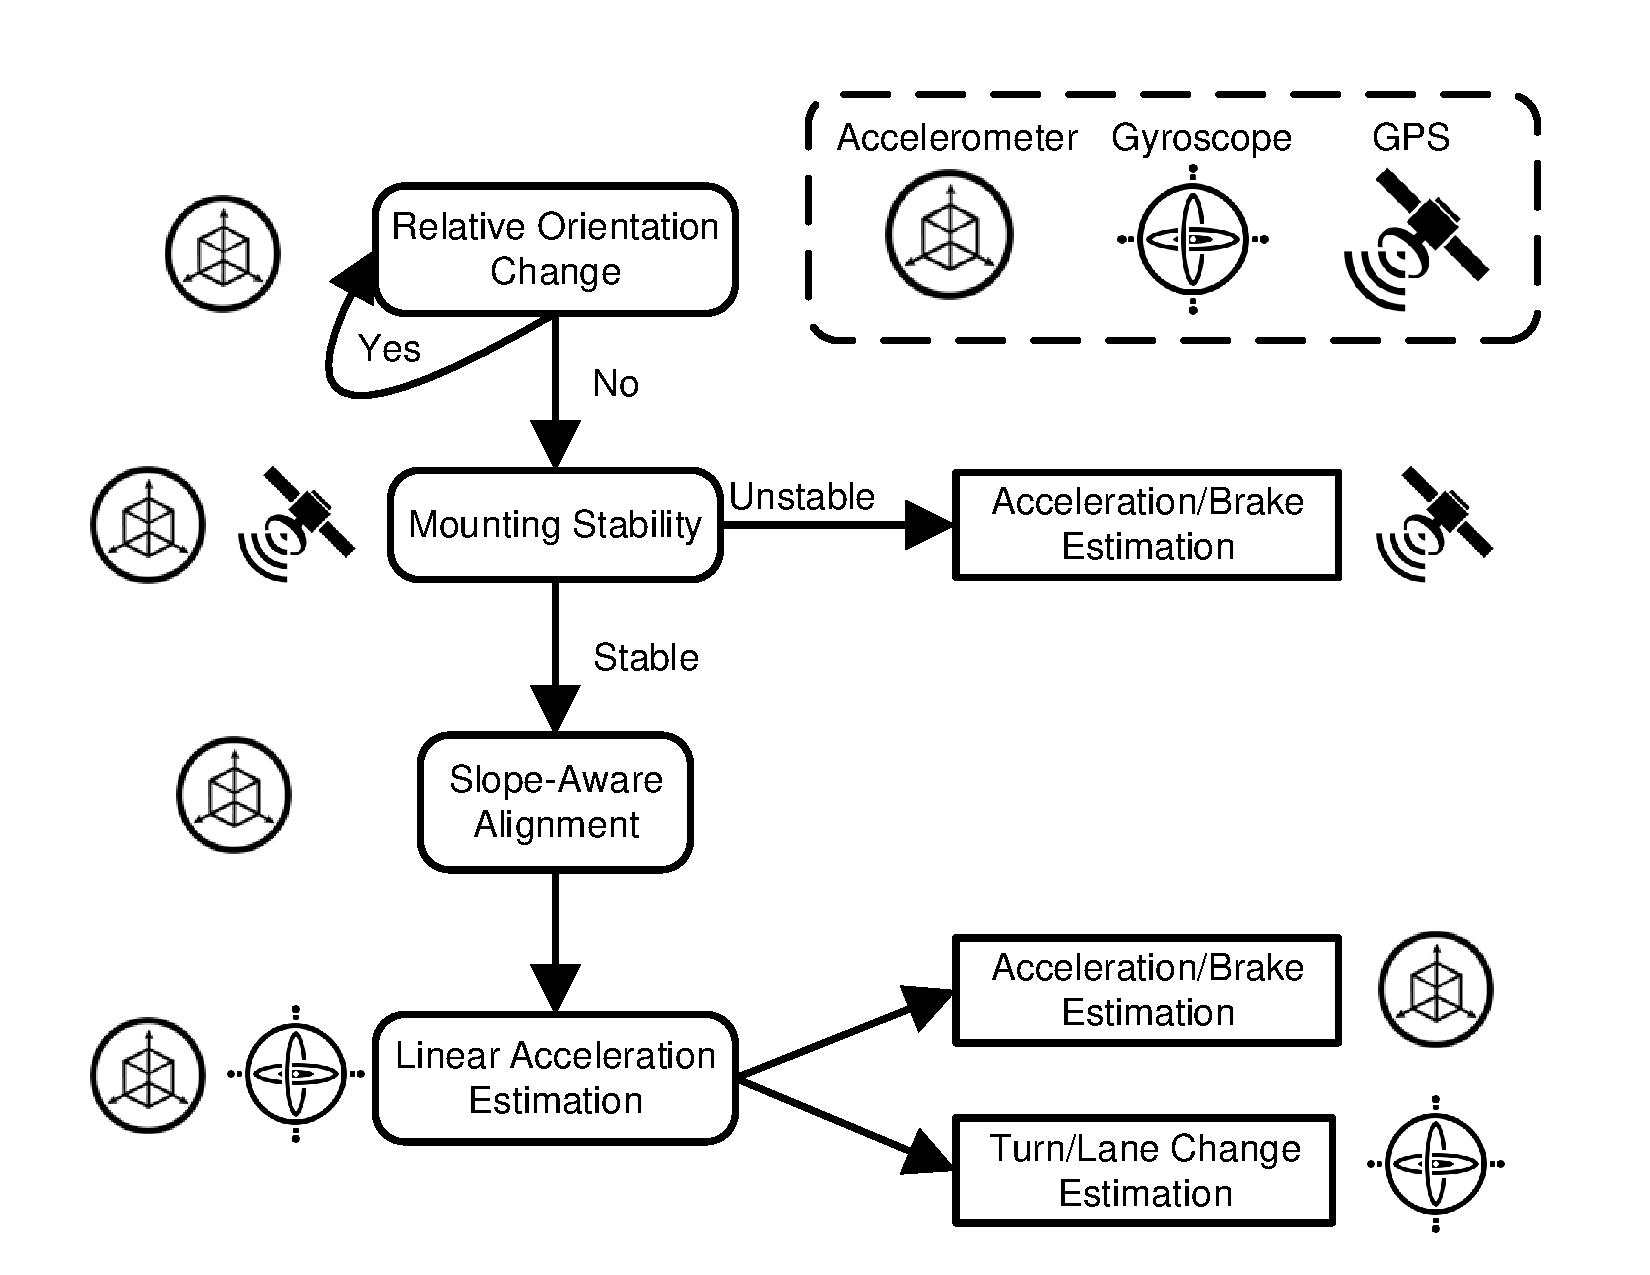
\includegraphics[width=3.6in, angle=0]{Figs/DriveSense/system_flowchart.pdf}
\vspace{-0.2cm}
\caption{Workflow of DriveSense.}
\vspace{-0.6cm}
\label{workflow}
\end{center}
\end{figure}


The workflow of DriveSense is illustrated in Fig. \ref{workflow}. 
DriveSense uses several modules to evaluate sensor
performance and estimate vehicle motion paramters. 
The inputs of DriveSense are accelerometer, gyroscope
and GPS.  
In each module, it uses different sensors as input.  
The corresponding sensor icon is placed along with the 
module if it requires that sensor as input.  
Our method uses the accelerometer extensively
as it provides a baseline by measuring the absolute acceleration while
the gyroscope measures only relative angular speed. 
The first module is to detect relative orientation changes.  
If an orientation change is detected, 
DriveSense will restart the rotation matrix
training process until the 
relative orientation of the phone is fixed.  
The second module is called stability monitoring
module, which is used to monitor the mounting
stability of the smartphone. 
The stability of the smartphone is quantified
by a threshold, which depends on the 
accuracy of GPS and that of the accelerometer. 
If the accuracy of the accelerometer is higher
than that of GPS, we think the smartphone
is mounted stably. 
In other case, we use GPS to estimate acceleration.
The third one is slope-aware coordinate
alignment module, 
which aligns the coordinates from the smartphone
to those of the car and estimates
the gradients of the training road segment. 
Both horizontal and vertical alignment are conducted
in this module. 
The last one is the linear acceleration estimation
module, which is used to estimate the slope 
gradients along the way.
DriveSense may selective use GPS or accelerometer
to estimate accelerations based on
the accuracy of each method. 
The accuracy comparison between GPS and accelerometer
is illustrated in section \ref{evaluation}. 



\subsubsection{Fusion with GPS}


GPS can be used to detect accelerations and brakes
when the IMU sensors are not available or not
ready to be used. 
IMU sensor is not available when the user 
frequently changes the relative orientation of the smartphone
or does not mount the smartphone stably. 
For example, if the user is holding the smartphone
to play game or send text message, 
the IMU sensor readings are too noisy 
to use. 
Even the user mounts the smartphone in a 
fixed place, it takes tens of seconds to minutes 
to collect enough data for training the rotation matrix. 
During the training process, the 
IMU sensors are not ready to be used.  
\footnote{The accelerometer takes much longer than gyroscope
as the gyroscope does not sense gravity.}


The GPS can also be used to eliminate the movement of the vehicle
when modeling mounting stability. 
We subtract the acceleration measured by the GPS from
the acceleration measured by the accelerometer. 
To do this, we project the 3D acceleration measured
by accelerometer into 2D space. 
Ideally, one dimension of senses gravity and the other
senses the horizontal movement of the car. 
For simplicity, we projects the 2D horizontal 
acceleration sensed by the accelerometer
into a single dimension and use it to subtract the acceleration
measured by GPS. 
We use this method only when the speed measured by GPS
is higher than a threshold. 


\subsection{Implementation}


We implement DriveSense as a software module in Java and 
import it to an Android application we wrote.
To make our test easier, we develop an offline 
trace replay engine.
The replay engine sorts the sensor data
based on timestamps, and feeds them into an event listener function in chronological order. 
We use an abstraction called \emph{Trace} to represent the sensor data, 
GPS data and OBD parameters.
It is similar to SensorEvent used by Android API \cite{sensor}
and provides additional flexibility to store OBD and GPS data. 
The event listener function process each \emph{Trace} 
according to corresponding sensor type.  
The trace replay engine makes it easier to import
DriveSense to the Android application. 
The Android application is aiming to monitor and record
daily driving trips. 
The app is implemented by less than 4,000 lines of Java code, 
but supports a variety of functionalities such as
trip recording, real time display, trip management,
trip display on Google map, user management and access control, 
online/offline uploading, data synchronization with remote server etc. 
DriveSense serves as a module that provide an more accurate
estimation on vehicle motions, e.g., hard brakes. 
For this submission, we highlight DriveSense module 
and remove some functionalities such as
trip upload, user management etc.
The QR code for a link to download the xsense.apk package is provided in Fig. \ref{xsense_app}. 

\begin{figure}[!tb]
\begin{center}
%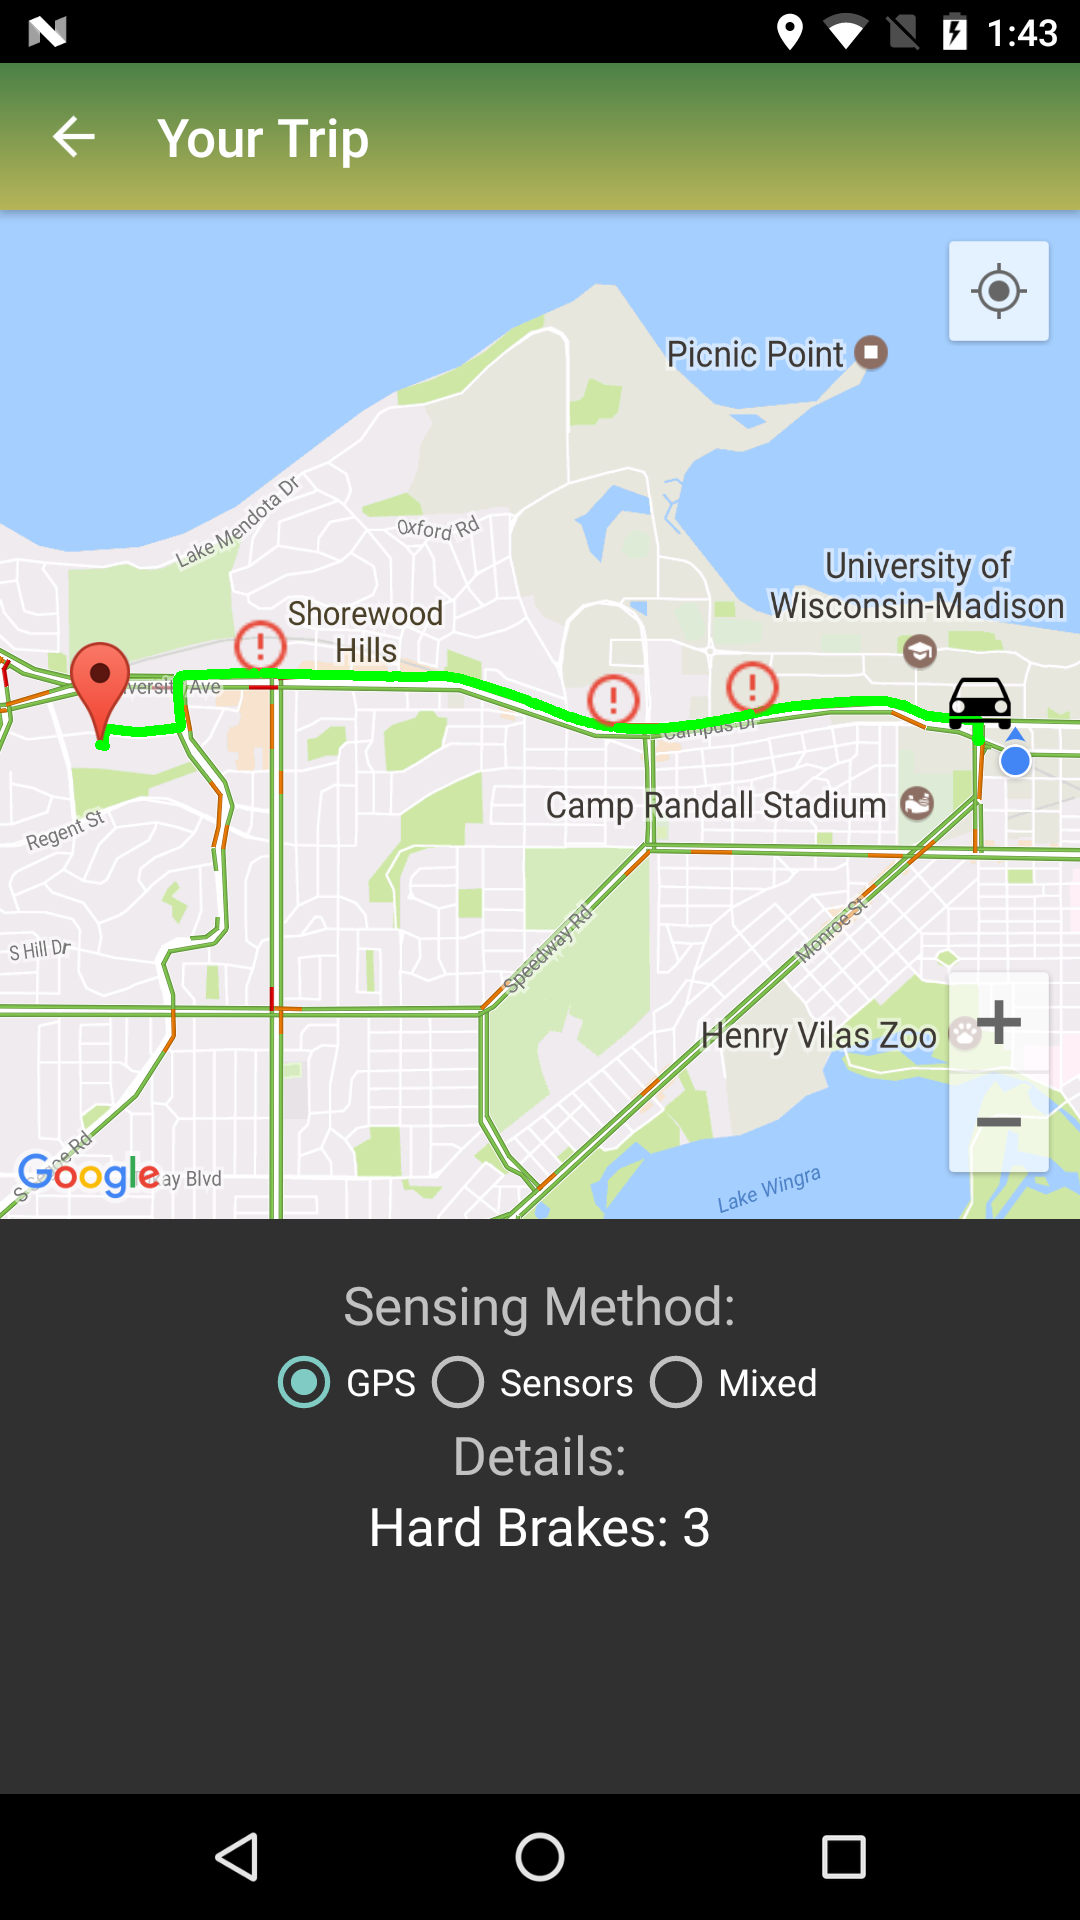
\includegraphics[width=1.7in,angle=0]{Figs/DriveSense/screenshot_gps.png}
%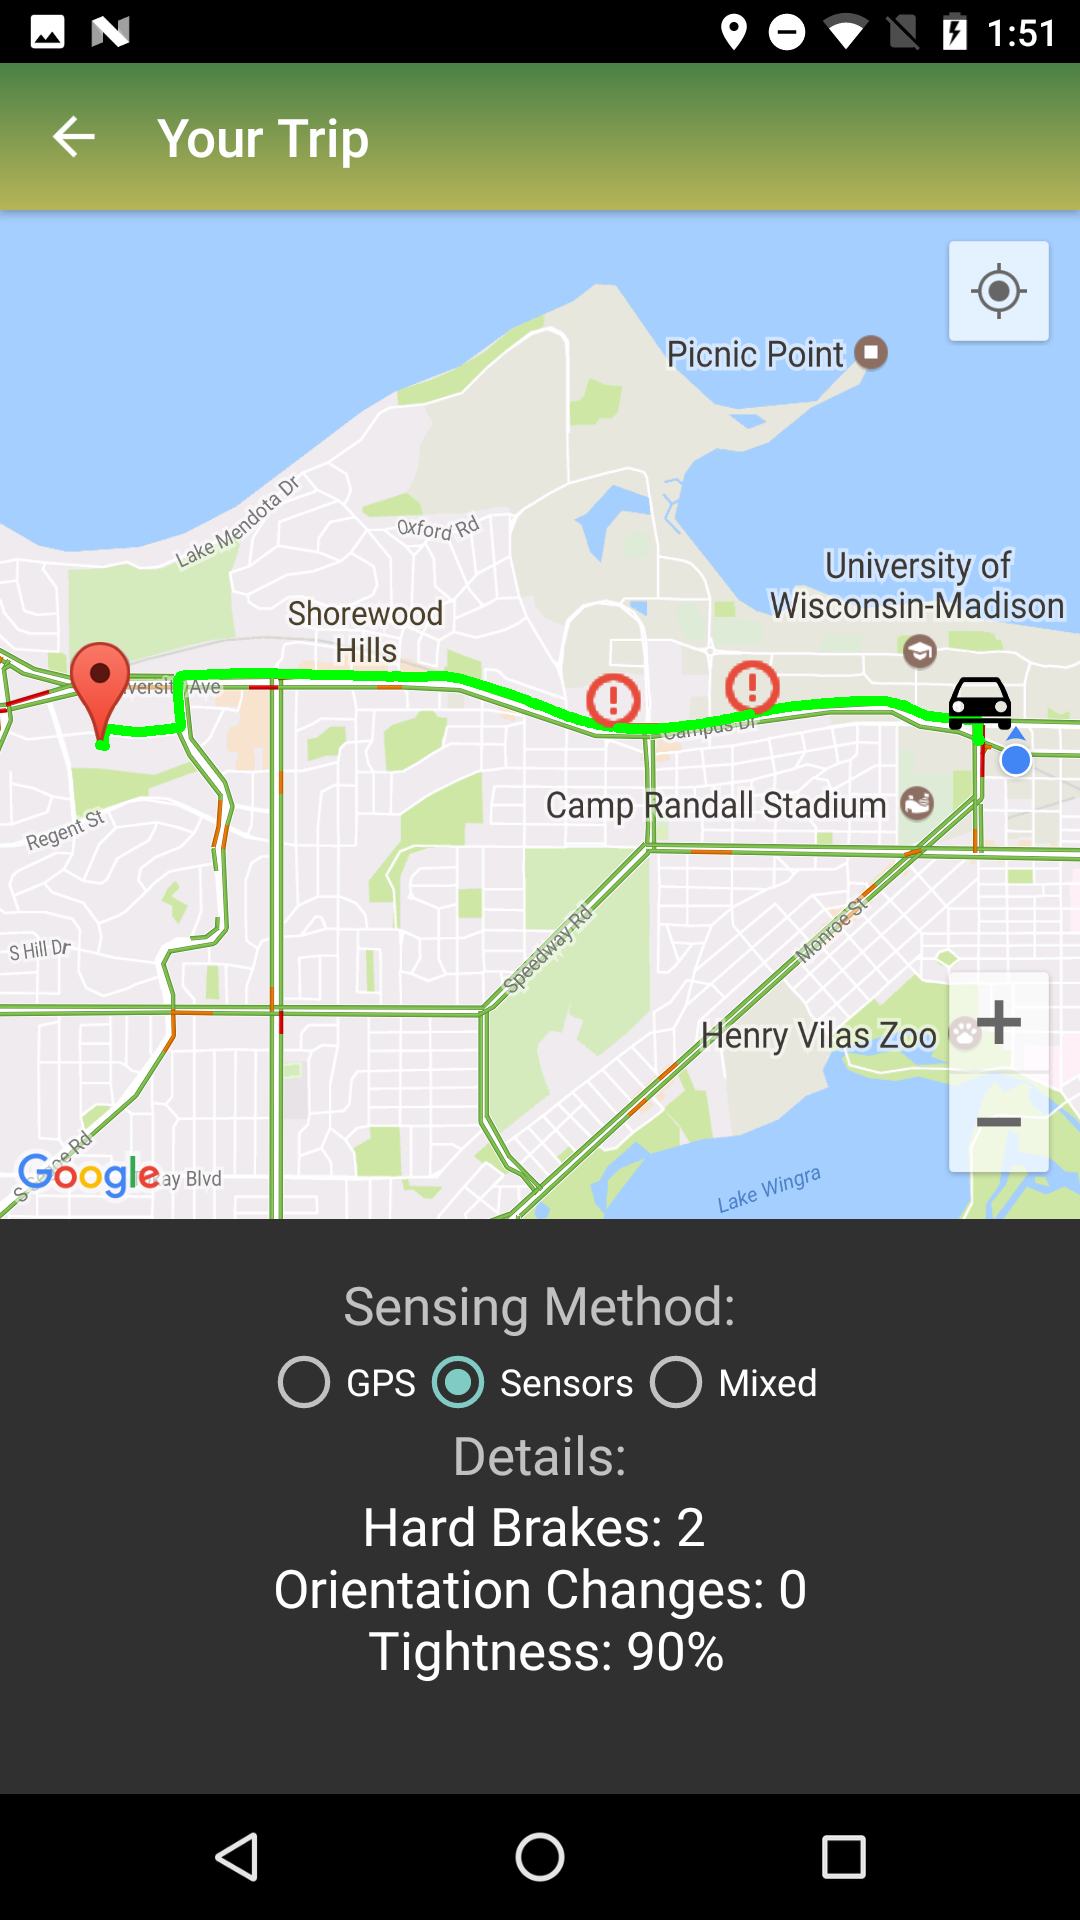
\includegraphics[width=1.7in,angle=0]{Figs/DriveSense/screenshot_sensors.png}
%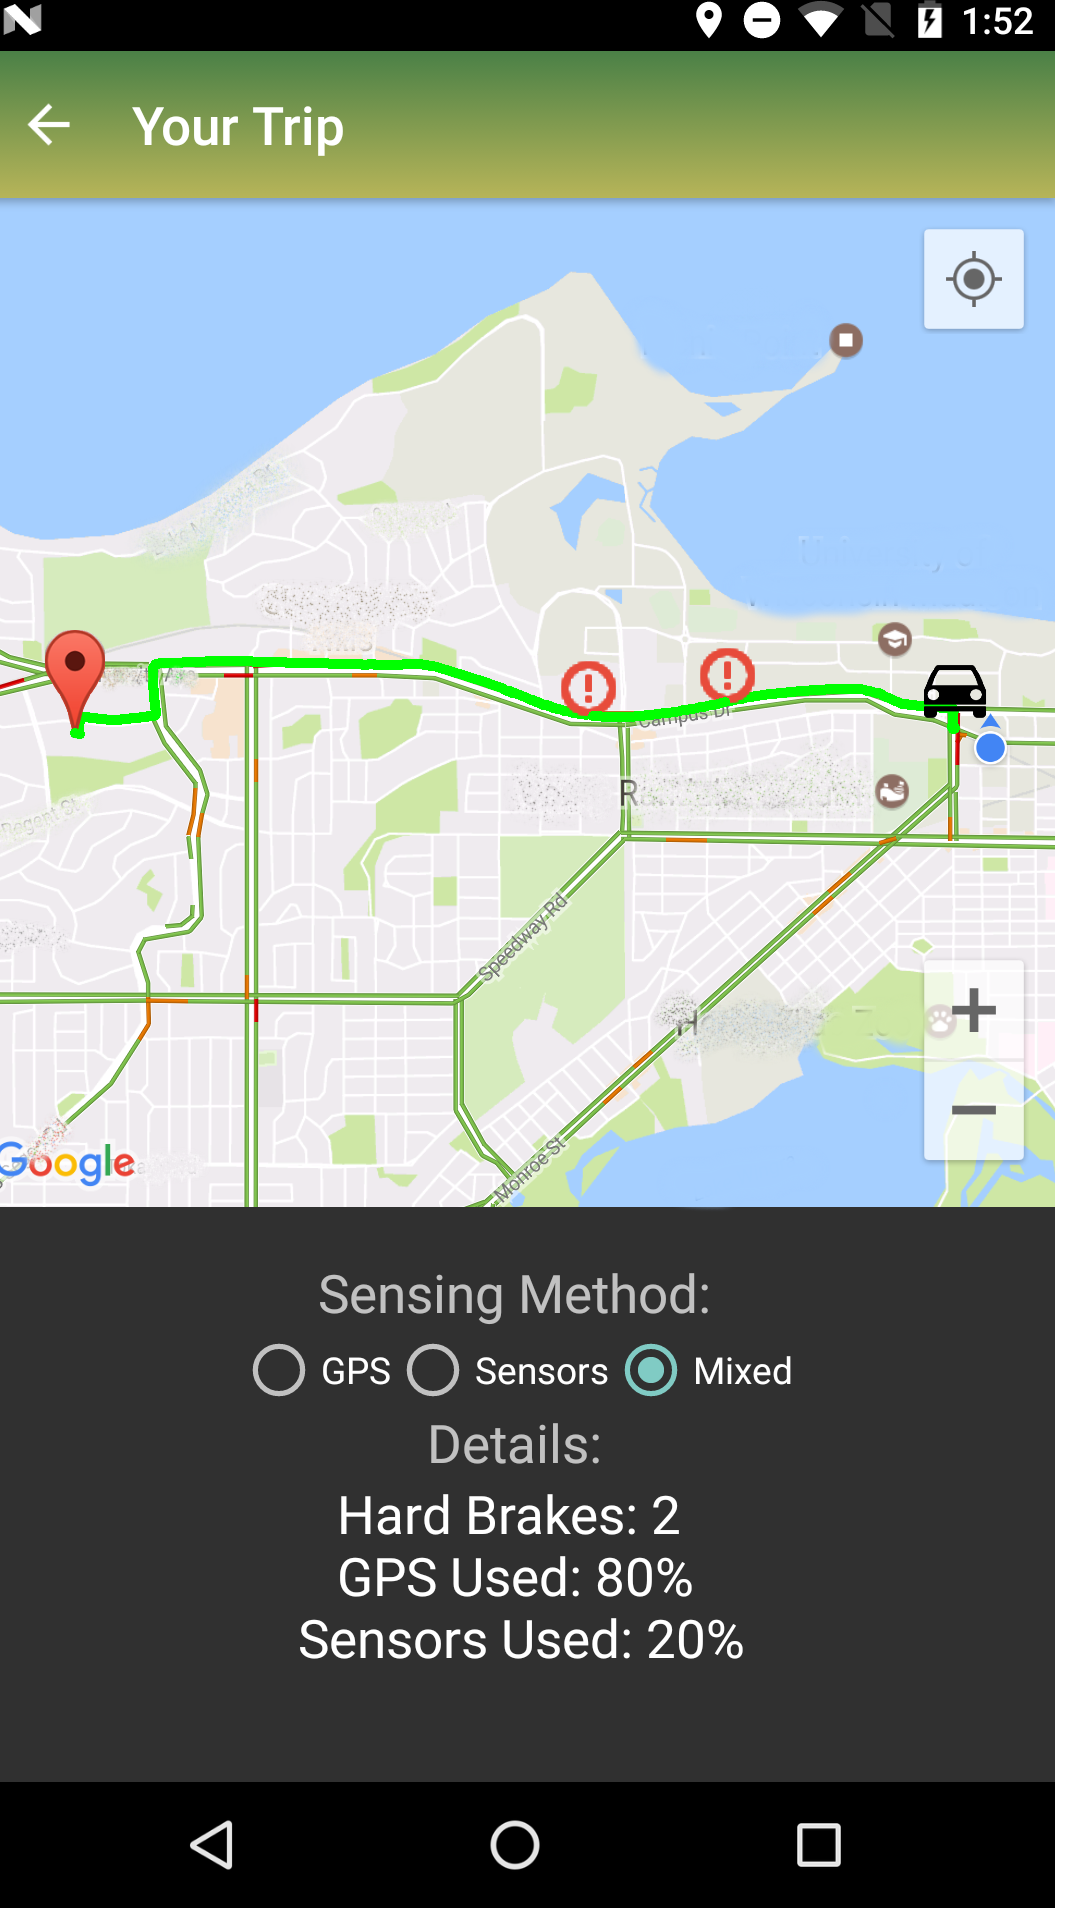
\includegraphics[width=1.8in, angle=0]{Figs/DriveSense/screenshot_mixed_hidden.png}
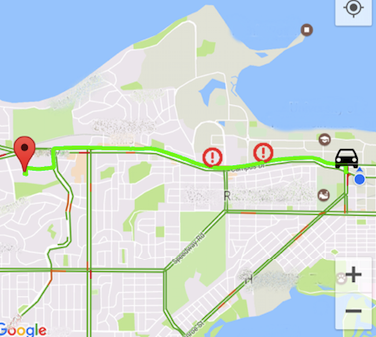
\includegraphics[width=1.8in, angle=0]{Figs/DriveSense/cut_app.png}
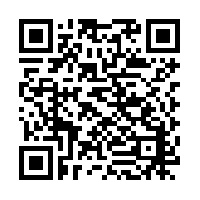
\includegraphics[width=1.4in, angle=0]{Figs/DriveSense/qrcode_xsense.png}
	\vspace{0.0cm}
\caption{The screenshot of DriveSense that user can view the hard brakes
	detected by GPS, sensors or mixed. The QR code can be scanned 
	to download the .apk Android installation file.}
\vspace{-0.2cm}
\label{xsense_app}
\end{center}
\end{figure}



